\section{外接球}

解决多面体外接球问题，难点是确定球心的位置，而要确定球心的位置，球的截面的性质起着关键的作用。

\subsection{外接球常用的性质}

\begin{theorem}{外接球}
    \begin{enumerate}
        \item 球心到截面（小圆）的距离 $d$ 与球的半径 $R$ 及截面的半径$r$有下面的关系：
              \[
                  R^2 = d^2 + r^2
              \]
        \item 过球心与小圆圆心的直线垂直于小圆所在的平面（类比：圆的垂径定理）
    \end{enumerate}
\end{theorem}

\subsection{长方体及其切割体模型}

\begin{figure} [H]
    \centering
    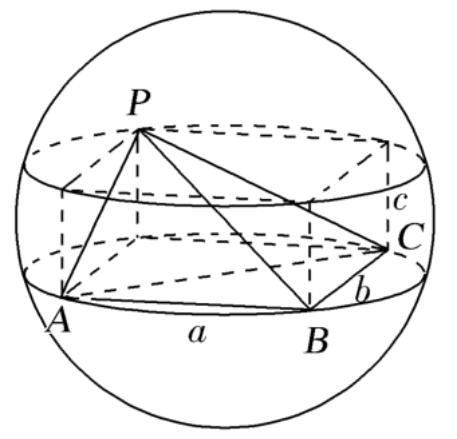
\includegraphics[width=0.2\textwidth]{chapters/立体几何/images/外接球/img-20250510030236.png}
    \caption{三棱锥的外接球就是长方体的外接球}
\end{figure}

\begin{example}
    在三棱锥$P-ABC$中，$PA$垂直$ABC$，$\angle BAC=90^\circ$，$PA=AB=AC=2$，则该三棱锥的外接球的表面积为 ( \hspace{1.5cm} )
    \begin{tasks}(4)
        \task $12\pi$
        \task $\frac{49\pi}{12}$
        \task $\frac{64\pi}{9}$
        \task $\frac{25\pi}{4}$
    \end{tasks}
\end{example}

\begin{example}
    三棱锥$P-ABC$的四个顶点都在球O的球面上，已知$PA$，$PB$，$PC$两两垂直，$PA=1$，$PB+PC=4$，当三角形的体积最大时，球O的体积为 ( \hspace{1.5cm} )
    \begin{tasks}(4)
        \task $36\pi$
        \task $9\pi$
        \task $\frac{9}{2}\pi$
        \task $\frac{9}{4}\pi$
    \end{tasks}
\end{example}

当然，并不是所有的题目都会很好心地给到明显的垂直，需要自己推理。

\vspace{0.5em}

\begin{example}
    已知三棱锥$P-ABC$的四个顶点在球$O$的球面上，$PA=PB=PC$，$\triangle ABC$是边长为$2$的正三角形，$E$，$F$分别是$PA$，$AB$的中点，$\angle CEF=90^\circ$，则球$O$的体积为 ( \hspace{1.5cm} )
    \begin{tasks}(4)
        \task $8\sqrt{6}\pi$
        \task $4\sqrt{6}\pi$
        \task $2\sqrt{6}\pi$
        \task $\sqrt{6}\pi$
    \end{tasks}
\end{example}

\begin{example}
    在正三棱锥$P-ABC$中，$PA \perp AB$，$P$到平面$ABC$的距离为$2$，则该三棱锥外接球的表面积为 ( \hspace{1.5cm} )
    \begin{tasks}(4)
        \task $36\pi$
        \task $16\pi$
        \task $\frac{16\pi}{3}$
        \task $4\pi$
    \end{tasks}
\end{example}

\subsection{另一类长方体：鳖臑（别闹）模型}

除了最明显的三垂直之外，还有可能出现类似这样的模型：

\begin{figure} [H]
    \centering
    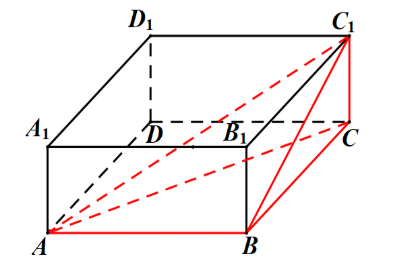
\includegraphics[width=0.3\textwidth]{chapters/立体几何/images/外接球/img-20250510033608.png}
\end{figure}


\begin{example}
    已知球$O$的面上有$A$、$B$、$C$、$D$四点，$DA \perp$ 面$ABC$，$AB \perp BC$，$DA = AB = BC = \sqrt{2}$，则球$O$的体积等于 ( \hspace{1.5cm} )
\end{example}

\vspace{8em}

\begin{example}
    三棱锥$P-ABC$中，$PA \perp$ 平面 $ABC$，$AC \perp BC$，$AC = BC = 1$，$PA = \sqrt{3}$，则该三棱锥外接球的表面积为 ( \hspace{1.5cm} )
    \begin{tasks}(4)
        \task $5\pi$
        \task $\sqrt{2}\pi$
        \task $20\pi$
        \task $4\pi$
    \end{tasks}
\end{example}

下面是一道需要思考立体几何证明性质的鳖臑模型：

\vspace{1em}

\begin{example}
    《九章算术·商功》：“斜解立方，得两导垂，斜解塔，其一为阳马，一为阵廊，阳马居二，阵廊居一，不易之难也。合两阵廊三而一，验之森，其形露矣。”即将底面为长方形且有一条与底面垂直的四棱锥称之为阳马，将四个面都为直角三角形的四面体称之为阵廊。如图所示为阵廊
    $V - ABC, \ V A \perp \text{平面}ABC, \ AB \perp BC, \ E, F \text{分别在棱} VB, VC \text{上, 且} EF \perp VC, \ AE \perp VB$.
    若$VA = 4$, 则三棱锥$V - AEF$外接球的体积为 ( \hspace{1.5cm} )

    \begin{figure} [H]
        \centering
        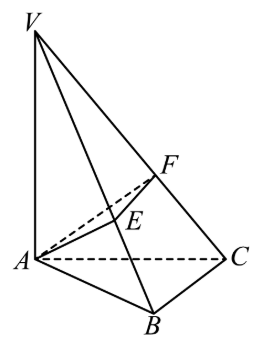
\includegraphics[width=0.2\textwidth]{chapters/立体几何/images/外接球/img-20250510034707.png}
    \end{figure}

    \begin{tasks}(4)
        \task $\frac{16}{3} \pi$
        \task $4\sqrt{2} \pi$
        \task $\frac{32}{3} \pi$
        \task $\frac{16\sqrt{2}}{3} \pi$
    \end{tasks}
\end{example}

\subsection{对棱相等的四面体模型}

\begin{example}
    正四面体的各条棱长均为 $\sqrt{2}$，则该正四面体外接球的体积为（\hspace{1.5cm}）
\end{example}

\begin{solution}
    本题是特殊情况，需要把这个四面体通过斜边相等的情况补全。如图，正四面体$A - B_1CD_1$的棱长为$\sqrt{2}$，把它补成正方体$ABCD - A_1B_1C_1D_1$，故正四面体$A - B_1CD_1$的外接球半径为$R = \frac{\sqrt{3}}{2}$.

    \[
        V_{\text{球}} = \frac{4}{3}\pi R^3 = \frac{4}{3}\pi \left( \frac{\sqrt{3}}{2} \right)^3 = \frac{\sqrt{3}\pi}{2}.
    \]

    \begin{figure} [H]
        \centering
        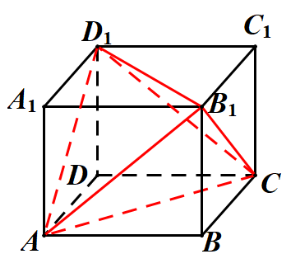
\includegraphics[width=0.3\textwidth]{chapters/立体几何/images/外接球/img-20250510035121.png}
    \end{figure}

\end{solution}

\begin{example}
    在四面体$A - BCD$中，$AB = CD = 5, \ AC = BD = \sqrt{34}, \ AD = BC = \sqrt{41}$，则四面体$A - BCD$外接球的表面积为（ \hspace{1.5cm} ）
    \begin{tasks}(4)
        \task $50\pi$
        \task $100\pi$
        \task $150\pi$
        \task $200\pi$
    \end{tasks}
\end{example}

\begin{example}
    在三棱锥$A - BCD$中，$AB = CD = 2,\ AD = BC = 3,\ AC = BD = 4$，则三棱锥$A - BCD$外接球的表面积为 \underline{\hspace{2cm}}。
\end{example}

\vspace{5em}

\begin{example}
    已知三棱锥$A - BCD$，三组对棱两两相等，且$AB = CD = 1,\ AD = BC = \sqrt{3}$，若三棱锥$A - BCD$的外接球表面积为$\frac{9\pi}{2}$，则$AC = \underline{\hspace{2cm}}$。
\end{example}

\subsection{涉及到立体展开图}

\begin{example}
    在正四面体$A - BCD$中，$E$是棱$AD$的中点，$P$是棱$AC$上一点，$BP + PE$的最小值为$\sqrt{7}$，则该正四面体的外接球的体积是（\hspace{1.5cm}）
    \begin{tasks}(4)
        \task $\sqrt{6}\pi$
        \task $6\pi$
        \task $\frac{3\sqrt{6}}{32}\pi$
        \task $\frac{3}{2}\pi$
    \end{tasks}
\end{example}

\begin{solution}
    将侧面$\triangle ABC$和$\triangle ACD$展开成平面图形，设正四面体的棱长为$a$，则$BP + PE$的最小值为
    \[
        BE = \sqrt{a^2 + a^2 - 2a \cdot \frac{1}{2} \cos 120^\circ} = \sqrt{7}, \quad a = \sqrt{7}, \quad \therefore a = 2.
    \]
    在正四面体$A - BCD$的边长为2，外接球的半径
    \[
        R = \frac{2}{4} = \frac{\sqrt{6}}{4}, \quad a = \frac{\sqrt{6}}{2}, \quad 外接球的体积 V = \frac{4}{3}\pi R^3 = 6\pi.
    \]
\end{solution}

\begin{example}
    如图所示，正四面体$ABCD$中，$E$是棱$AD$的中点，$P$是棱$AC$上一点，$BP + PE$的最小值为$\sqrt{14}$，则该正四面体的外接球表面积是（\hspace{1.5cm} ）
    \begin{tasks}(4)
        \task $12\pi$
        \task $32\pi$
        \task $8\pi$
        \task $24\pi$
    \end{tasks}
\end{example}

\newpage{}

\subsection{阶段性习题}

\begin{enumerate}
    \item 如图，已知球的球心为$O$，$B, C, D, A$四点在球面上，$DA \perp$ 平面 $ABC$，且 $AB \perp BC$，$DA = AB = BC = \sqrt{2}$，球的体积等于\underline{\hspace{2cm}}。

    \item 已知四面体 $P - ABC$ 四个顶点都在球 O 的球面上，若$PB \perp$ 平面  $ABC$，且$AB \perp AC$，$AB = PB = 2$，则球的表面积为\underline{\hspace{2cm}}。

    \item 已知三棱锥$S - ABC$中，$SA = BC = \sqrt{13}$，$SB = AC = \sqrt{5}$，$SC = AB = \sqrt{10}$，则三棱锥的外接球的表面积为\underline{\hspace{2cm}}。

    \item 在古代将四个面都为直角三角形的四面体称之为鳖臑，已知四面体$A - BCD$为鳖臑，$AB \perp \text{平面}BCD$，且$AB = BC = \frac{\sqrt{3}}{6}CD$，若此四面体的体积为$\frac{8\sqrt{3}}{3}$，则其外接球的表面积为\underline{\hspace{2cm}}。

    \item 在长方体$ABCD - A_1B_1C_1D_1$中，底面$ABCD$是边长为$3\sqrt{2}$的正方形，$AA_1 = 3$，$E$是线段$A_1B_1$上一点，若第二面角$A - BD - E$的正切值为3，则三棱锥$A - A_1D_1E$外接球的表面积为\underline{\hspace{2cm}}。

    \item 在三棱锥$A - BCD$中，$AB = CD = 6$，$AC = BD = AD = BC = 5$，则该三棱锥的外接球的体积为\underline{\hspace{2cm}}。

    \item 已知四面体$ABCD$满足$AB = CD = \sqrt{6}$，$AC = AD = BC = BD = 2$，则四面体$ABCD$的外接球的表面积是\underline{\hspace{2cm}}.

\end{enumerate}

\subsection{直棱柱模型}
\begin{theorem}{直棱柱外接球}
    设直棱柱$ABC - A_1B_1C_1$的高$CC_1 = h$。由对称性可知球心$O$的位置是$\triangle ABC$的外心$O_1$与$\triangle A_1B_1C_1$的外心$O_2$连线的中点，设小圆$O_1$的半径$AO_1 = r$，又$OO_1 = \frac{h}{2}$，因此有：
    \[
        R^2 = r^2 + \frac{h^2}{4}.
    \]

    \begin{figure} [H]
        \centering
        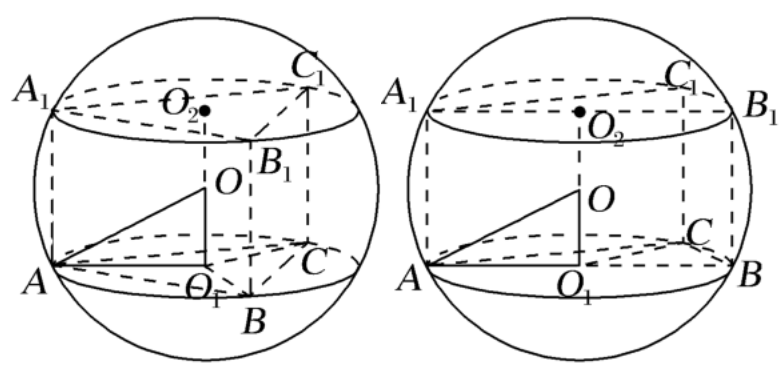
\includegraphics[width=0.4\textwidth]{chapters/立体几何/images/外接球/img-20250510052133.png}
    \end{figure}
\end{theorem}

\pagebreak

\begin{example}
    已知直三棱柱$ABC - A_1B_1C_1$的6个顶点都在球$O$的球面上。若$AB = 3$，$AC = 4$，$AB \perp AC$，$AA_1 = 12$，则球$O$的半径为（ \hspace{1.5cm}）
    \begin{tasks}(4)
        \task $\frac{3\sqrt{17}}{2}$
        \task $2\sqrt{10}$
        \task $\frac{13}{2}$
        \task $3\sqrt{10}$
    \end{tasks}
\end{example}

\v{8em}

其中，底面三角形的外接圆半径如果不好直接求解（如直角三角形的外接圆圆心刚好在斜边的中点，这是好判断的），可以用正弦定理来处理。

\begin{example}
    三棱锥$S - ABC$中，侧棱$SA \perp$ 底面$ABC$，$AB = 5$，$BC = 8$，$\angle B = 60^\circ$，$SA = 2\sqrt{5}$，则该三棱锥的外接球的表面积为（ \hspace{1.5cm}）
    \begin{tasks}(4)
        \task $\frac{64}{3}\pi$
        \task $\frac{256}{3}\pi$
        \task $\frac{436}{3}\pi$
        \task $\frac{2048}{27}\sqrt{3}\pi$
    \end{tasks}
\end{example}

\v{8em}

\begin{example}
    在三棱锥$P - ABC$中，已知$PA \perp$ 底面$ABC$，$\angle BAC = 120^\circ$，$PA = AB = AC = 2$，若该三棱锥的顶点都在同一个球面上，则该球的表面积为（\hspace{1.5cm} ）
    \begin{tasks}(4)
        \task $10\sqrt{3}\pi$
        \task $18\pi$
        \task $20\pi$
        \task $9\sqrt{3}\pi$
    \end{tasks}
\end{example}

\v{8em}

\begin{example}
    在三棱锥$P - ABC$中，$PA \perp$ 平面$ABC$，$\angle BAC = 120^\circ$，$AC = 2$，$AB = 1$，设$D$为$BC$中点，且直线$PD$与平面$ABC$所成的余弦值为$\frac{\sqrt{5}}{5}$，则该三棱锥外接球的表面积为（\hspace{1.5cm}）
\end{example}

\v{8em}

\begin{example}
    在三棱锥$P - ABC$中，平面$PAC \perp$ 平面$ABC$，$AB \perp AC$，$PA = PC = AC = 2$，$AB = 4$，则三棱锥$P - ABC$的外接球的表面积为（ \hspace{1.5cm}）
    \begin{tasks}(4)
        \task $23\pi$
        \task $\frac{23}{4}\pi$
        \task $64\pi$
        \task $\frac{64}{3}\pi$
    \end{tasks}
\end{example}

% \subsection{}


% 注意在公式环境中出现文字时需要用 \text{} 包裹起来，另外，你读到什么内容就写什么内容，不要轻易修改我的文字、数据、表述。请返回给我一个 LateX 代码块